\documentclass[sigconf]{acmart}

\usepackage{amsmath}
\usepackage{xcolor}
\usepackage{booktabs}
\usepackage{listings}
\usepackage{framed}
\usepackage{graphicx}
\graphicspath{{Figures/}}

\lstset{
  basicstyle=\ttfamily\footnotesize,
  columns=fullflexible,
  keepspaces=true,
  showstringspaces=false,
  breaklines=true,
  breakatwhitespace=true,
  tabsize=2
}

\setcopyright{none}
\settopmatter{printacmref=false}
\acmDOI{}
\acmISBN{}
\acmConference[Draft '26]{Draft ACM-Style Conference Submission}{2026}{TBD}
\acmYear{2026}
\copyrightyear{2026}

\title{AURIS: An LLM-Driven Framework for Structured Mental Health Assessment Using Mixture-of-Experts Architecture}

\author{Tristan James Y. Tolentino}
\affiliation{%
  \institution{Cebu Institute of Technology - University}
  \city{Cebu City}
  \country{Philippines}
}
\email{tristanjamestolentino56@gmail.com}

\author{Julia Laine G. Segundo}
\affiliation{%
  \institution{Cebu Institute of Technology - University}
  \city{Cebu City}
  \country{Philippines}
}
\email{julialaine.segundo@cit.edu}

\author{Adrian T. Sajulga}
\affiliation{%
  \institution{Cebu Institute of Technology - University}
  \city{Cebu City}
  \country{Philippines}
}
\email{adrian.sajulga@cit.edu}

\author{Jun Albert S. Pardillo}
\affiliation{%
  \institution{Cebu Institute of Technology - University}
  \city{Cebu City}
  \country{Philippines}
}
\email{junalbert.pardillo@cit.edu}

\renewcommand{\shortauthors}{Tolentino et al.}

\begin{abstract}
AURIS targets the mental health treatment gap with a retrieval-augmented, safety-aware conversational assessor. Built on the LLaMA 4 Scout mixture-of-experts model and a RAG pipeline, it adapts 14 validated questionnaires (178 items) across three phases: Rapport, Screening, and Snapshot. Using the ESHRO hybrid evaluation (automated metrics plus expert review), AURIS achieved a 0.76 composite score; human raters scored Safety at 1.00 and Empathy at 0.88, while automated relevance lagged at 0.53, highlighting that standard similarity metrics miss clinical alignment. The system is a preventive psychiatry prototype---an empathetic, low-friction first touchpoint rather than a therapy replacement. Future work includes domain-specific fine-tuning and clinically grounded automated metrics.
\end{abstract}

\begin{CCSXML}
<ccs2012>
 <concept>
  <concept_id>10002951.10003227.10003236.10003237</concept_id>
  <concept_desc>Information systems~Data mining</concept_desc>
  <concept_significance>300</concept_significance>
 </concept>
 <concept>
  <concept_id>10010147.10010257.10010293</concept_id>
  <concept_desc>Computing methodologies~Natural language generation</concept_desc>
  <concept_significance>500</concept_significance>
 </concept>
 <concept>
  <concept_id>10003120.10003145.10003151</concept_id>
  <concept_desc>Human-centered computing~Interaction design</concept_desc>
  <concept_significance>100</concept_significance>
 </concept>
</ccs2012>
\end{CCSXML}

\ccsdesc[500]{Computing methodologies~Natural language generation}
\ccsdesc[300]{Information systems~Data mining}
\ccsdesc[100]{Human-centered computing~Interaction design}

\keywords{Large Language Models (LLMs), LLaMA 4 Scout, Retrieval-Augmented Generation (RAG), Mental Health Screening, ESHRO Framework, Preventive Psychiatry, Conversational Agents, Clinical Assessment}

\begin{document}
\maketitle
\section{Introduction}
Mental health conditions remain widespread yet under-treated because of stigma, cost, and clinician shortages \cite{1,2}. Talk therapy is still the efficacy benchmark \cite{3,21}, but many people delay care until impairment is severe \cite{2}. To widen access, we explore a digital assistant that keeps clinical structure while reducing friction.

Recent work shows Large Language Models (LLMs) can deliver empathetic, context-aware support \cite{4,5,6,7}, though safety and alignment vary by architecture and training \cite{8}. We build on LLaMA 4 Scout---a mixture-of-experts model with long-context support \cite{9,10,11}---to create AURIS, a retrieval-augmented, safety-aware assessor aimed at preventive psychiatry rather than replacing therapy \cite{1,22}.

\section{Related Work}
LLM use in mental health is expanding but constrained by privacy and terminology issues \cite{12}, even as newer multimodal, high-capacity models (e.g., the Llama 4 herd) improve reasoning and context handling \cite{11}. Evidence syntheses note strong capabilities alongside safety variation \cite{4,5,6,7,8,20}.

Recent systems move beyond general models: ZhiXin fine-tunes Llama on clinical records \cite{12}; Milo adapts CBT for teens \cite{13}; FlexiDialogue replaces rigid trees with instruction-driven flows \cite{14}; SouLLMate combines RAG and prompt design for guidance and risk detection \cite{15}. Reviews group applications into screening, treatment support, and counseling \cite{5}, with new work on automated intake \cite{16} and on coping with heterogeneous instruments \cite{17}.

Evaluation remains challenging: ESHRO scores empathy, safety, helpfulness, and relevance \cite{18}; CounseLLMe compares AI--human dialogue patterns \cite{19}. Risks include hallucinations, privacy, and fairness \cite{8,20}. The treatment gap persists \cite{2}, talk therapy is still the benchmark \cite{3,21}, and many advocate a preventive stance where digital tools augment care without medicalizing well-being \cite{1,22}.

\section{Methodology}
This section details the methodological design of AURIS, a retrieval-augmented, safety-aware clinical screening system for structured mental health assessment. We summarize the RAG pipeline, questionnaire integration, schema design, state management, evaluation methodology, and safety handling.

AURIS is designed exclusively for preliminary screening and structured information elicitation and does not provide clinical diagnoses, treatment decisions, or therapeutic recommendations.

\begin{figure}[htbp]
\centering
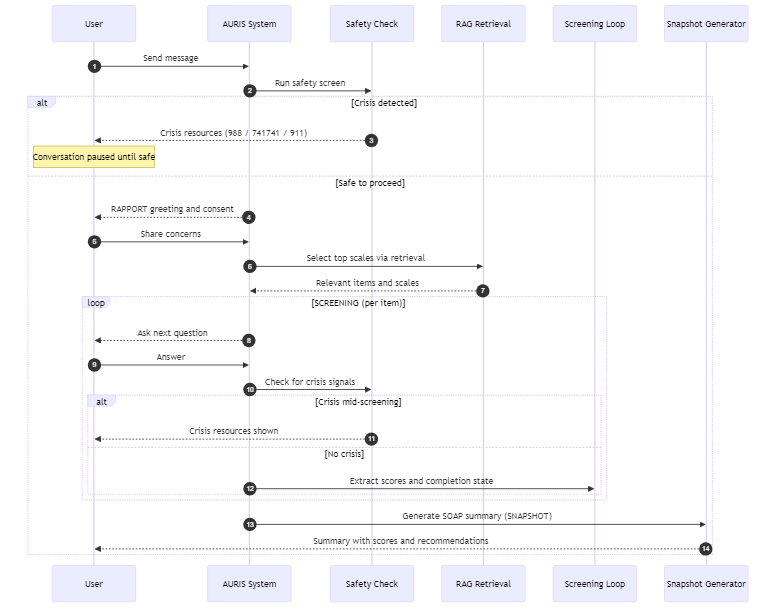
\includegraphics[width=0.8\textwidth]{workflow.png}
\Description{System workflow diagram showing the end-to-end AURIS assessment pipeline from user input through retrieval, screening flow, and structured clinical snapshot output.}
\caption{End-to-end AURIS workflow from user input to structured clinical snapshot}
\label{fig:workflow}
\end{figure}

\subsection{Retrieval-Augmented Generation (RAG) Pipeline}
AURIS employs a retrieval-augmented generation (RAG) approach to dynamically select clinically relevant assessment items in response to user inputs. Text embeddings are generated using the \texttt{sentence-transformers/all-MiniLM-L6-v2} model, producing 128-dimensional vectors optimized for semantic similarity tasks \cite{23}. These embeddings are persistently stored in ChromaDB, with cosine similarity used to retrieve the top-$k$ ($k = 5$) most relevant items per query.

Each query embedding is constructed from a composite input consisting of the last three conversational turns and a large language model (LLM)-generated concern summary, enabling contextual continuity across interactions.

To improve recall across heterogeneous user language styles, dual embeddings are maintained for each questionnaire item: one embedding derived from the formal clinical phrasing and another derived from colloquial semantic hook phrases. This dual-representation strategy balances clinical fidelity with accessibility to non-expert users.

To reduce redundancy across overlapping diagnostic instruments (e.g., sleep-related items shared by GAD-7 and ISI), an overlap detection module identifies the top-2 most relevant scales and injects discriminatory prompts designed to elicit differentiating symptoms. Retrieved items propagate their metadata---including \texttt{scale\_id}, \texttt{item\_id}, \texttt{domain}, \texttt{scoring\_rules}, \texttt{severity\_thresholds}, and \texttt{is\_critical} flags---through all downstream pipeline stages.

\subsection{Clinical Questionnaires and Instrument Coverage}
The system integrates fourteen validated clinical questionnaires, comprising a total of 178 individual items, covering the domains of depression, anxiety, PTSD, sleep disturbance, perceived stress, substance use, ADHD, OCD, social anxiety, burnout, bipolar disorder screening, and eating disorders \cite{24,25,26,27,28,29,30,31,32,33,34,35,36,37}.

Questionnaire items, scoring rules, reverse-scoring flags, and severity thresholds were programmatically extracted using Gemini 3 Thinking, followed by manual verification against original instrument publications. Severity classifications strictly follow published cutoffs; for example, PHQ-9 severity ranges are defined as minimal (0--4), mild (5--9), moderate (10--14), moderately severe (15--19), and severe (20--27) \cite{4}.

Items associated with acute risk, including suicidal ideation (e.g., PHQ-9 Item 9), self-harm, and severe substance misuse, are explicitly marked as \texttt{is\_critical} and routed to predefined rule-based safety handling pathways. Full questionnaire inventories, scoring exemplars, and structured JSON representations are provided in Appendix A, while extraction and transformation prompts are detailed in Appendix B.

\subsection{Schema Design and Data Compression}
To ensure consistency and scalability, AURIS defines a standardized JSON schema encompassing the following required fields: unique identifiers, clinical text, semantic hooks, scoring logic, reverse-scoring indicators, criticality flags, diagnostic domains, and severity thresholds.

A hook-based semantic compression strategy is employed, wherein each item is represented by 3--5 word semantic units capturing its diagnostic intent. Combined with metadata minification and removal of redundant lexical content, this approach achieves an average 73\% reduction in dataset size, compressing the full questionnaire corpus from 299 KB to 80 KB for 178 items.

All records are stored in JSON Lines (\texttt{jsonl}) format to facilitate streaming ingestion and efficient embedding generation. Schema compliance is enforced using \texttt{jsonschema} validation to guarantee structural integrity and type correctness at load time. Sample compressed records and reverse-scoring implementations are presented in Appendix A.

\subsection{System Architecture and State Management}
AURIS follows a three-phase interaction model: \textbf{RAPPORT} (trust and context building), \textbf{SCREENING} (adaptive RAG-driven assessment), and \textbf{SNAPSHOT} (structured clinical summarization).

Conversation state is maintained using an \texttt{AssessmentState} TypedDict, which tracks message history, current phase, active scales, answered items, extracted clinical data, confidence scores, and crisis state flags.

\begin{figure}[htbp]
\centering
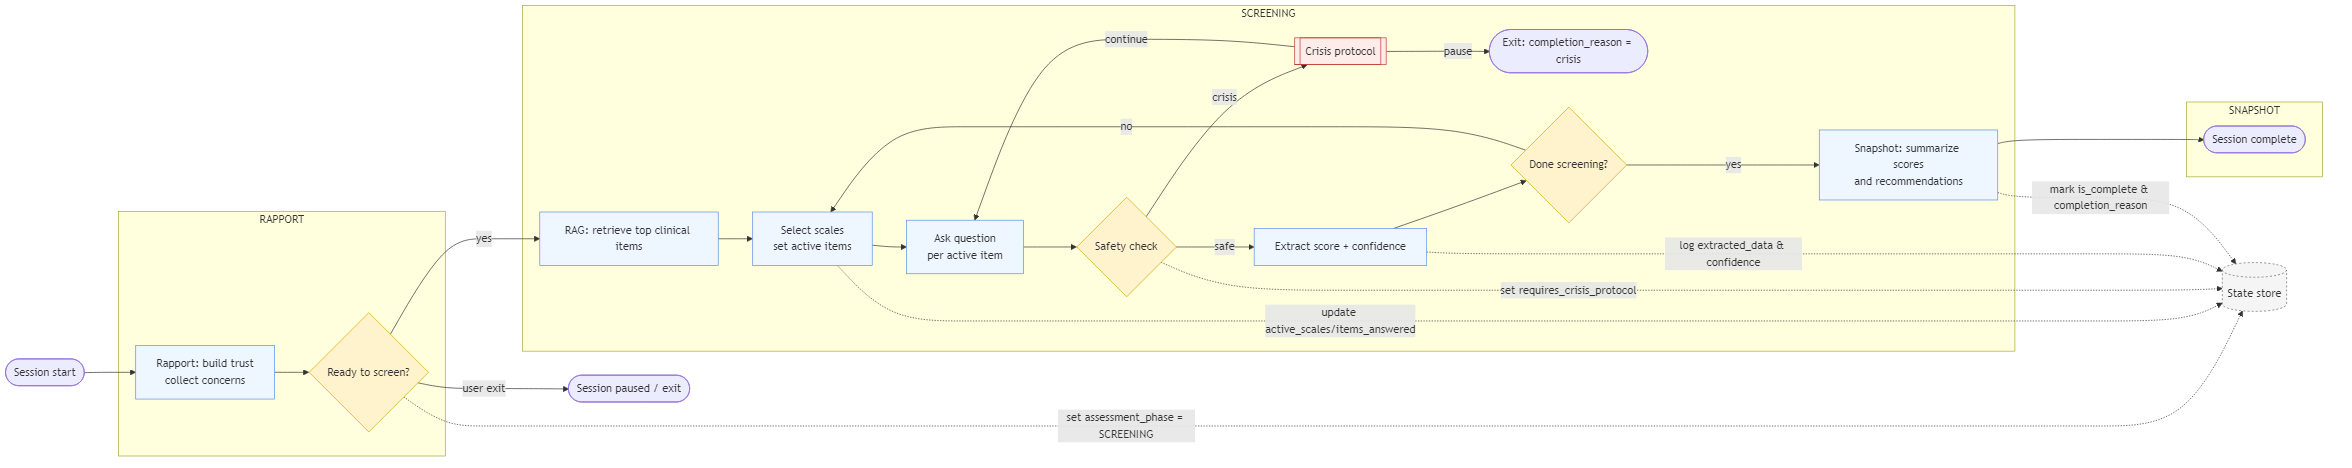
\includegraphics[width=0.8\textwidth]{fig2.png}
\Description{Architecture diagram of the RAG-driven screening process, including phase transitions, state tracking, retrieval, overlap handling, and summary generation.}
\caption{RAG-driven screening pipeline, phase transitions, and state management}
\label{fig:pipeline}
\end{figure}

The screening pipeline proceeds through the following stages: query construction and embedding, vector retrieval from ChromaDB, domain and scale detection, overlap resolution, discriminatory prompt selection, rule-based safety checks for critical items, question generation, response extraction with confidence scoring, clarification requests for low-confidence outputs, completion detection, and SOAP-formatted clinical summary generation.

Additional implementation artifacts (e.g., prompt templates) are available upon request.

\subsection{Evaluation Framework: ESHRO Hybrid Scoring}
System performance is evaluated using the ESHRO hybrid evaluation framework \cite{18}, combining automated metrics with LLM-based human proxy assessment.

\begin{figure}[htbp]
\centering
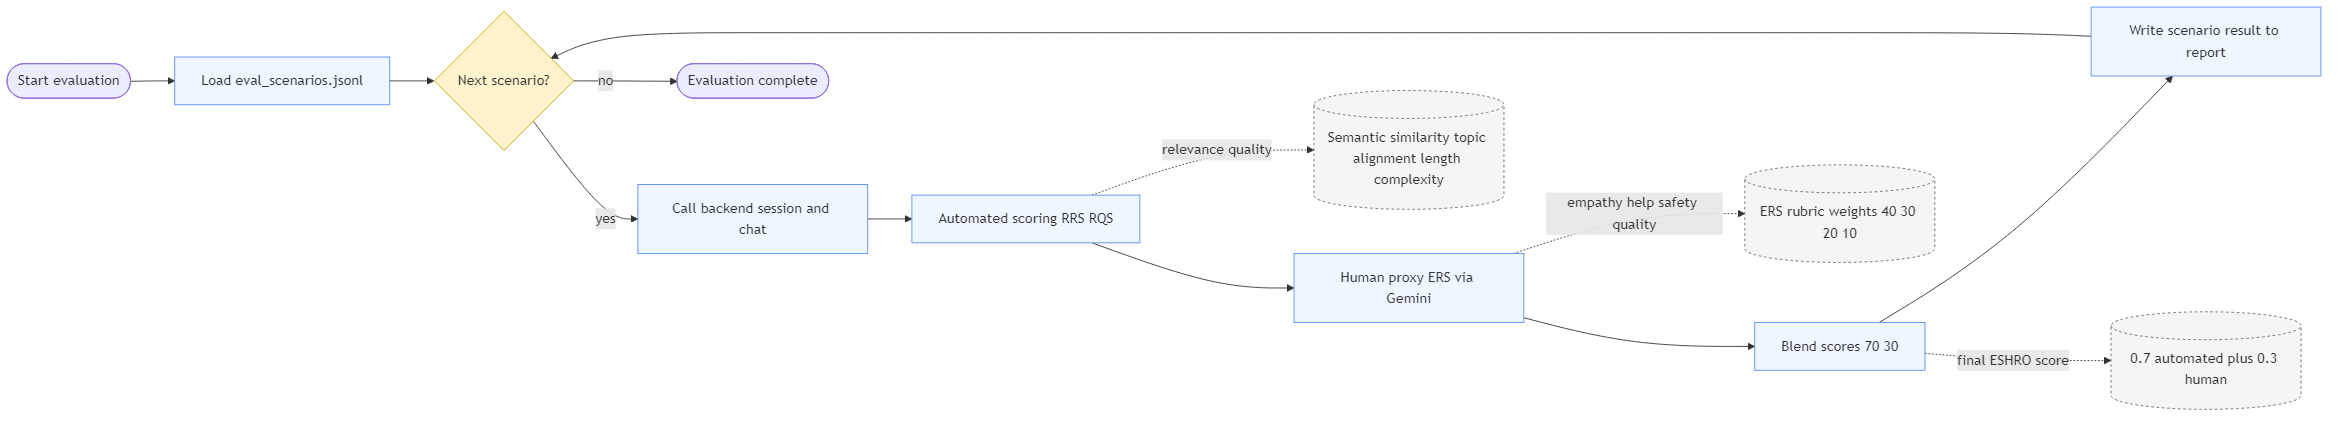
\includegraphics[width=0.8\textwidth]{fig3.png}
\Description{Evaluation and safety diagram showing the ESHRO scoring components and crisis-safety enforcement in the assessment workflow.}
\caption{ESHRO evaluation framework and safety enforcement integration}
\label{fig:eshro}
\end{figure}

Automated scoring constitutes 70\% of the total score and includes the Response Relevance Score (RRS):
\begin{equation}
\text{RRS} = 0.6 \times \text{SemanticSim} + 0.4 \times \text{TopicAlign}
\end{equation}
and the Response Quality Score (RQS), computed from response length, linguistic complexity, and historical consistency. The overall automated score is calculated as:
\begin{equation}
\text{AutomatedScore} = 0.5 \times \text{RRS} + 0.5 \times \text{RQS}
\end{equation}

Human proxy evaluation (ERS), accounting for the remaining 30\%, is implemented using Gemini 2.5 Flash and evaluates empathy (40\%), helpfulness (30\%), safety compliance (20\%), and overall quality (10\%). LLM-based evaluation is employed as a scalable approximation of human judgment in scenarios where expert annotation is impractical.

\subsection{Safety and Crisis Handling}
Safety enforcement is integrated throughout the screening and summarization stages. Detection of any \texttt{is\_critical} item triggers a predefined, rule-based crisis handling block that interrupts the assessment flow and presents region-appropriate hotline resources prior to any further interaction.

Users retain autonomy to continue, pause, or exit the assessment. Supplementary prompt and scenario details are available upon request.

\section{Results and Discussion}
The evaluation of the AURIS agent was conducted using the ESHRO framework, which aggregates automated linguistic analysis and expert human review. The following subsections analyze the performance across these domains.

\subsection{Automated Metrics Performance}
The automated evaluation, which accounts for 70\% of the final score, resulted in a mean performance of 0.71. This metric is further divided into Relevance (RRS) and Quality (RQS).

\begin{table}[htbp]
\caption{ESHRO Evaluation Summary}
\begin{center}
\begin{tabular}{lc}
\toprule
\textbf{Metric} & \textbf{Score} \\
\midrule
Automated Relevance (RRS) & 0.53 \\
Automated Quality (RQS) & 0.89 \\
\textbf{Overall Automated Score} & \textbf{0.71} \\
\midrule
Human Empathy (ERS) & 0.88 \\
Human Helpfulness (ERS) & 0.75 \\
Human Safety (ERS) & 1.00 \\
\textbf{Overall Human Score} & \textbf{0.88} \\
\midrule
\textbf{Final ESHRO Score} & \textbf{0.76} \\
\bottomrule
\end{tabular}
\label{table1}
\end{center}
\end{table}

As shown in Table~\ref{table1}, the agent achieved high Quality scores (0.89) but lower Relevance scores (0.53). This indicates that while responses are generally well-formed, they can deviate from the specific semantic expectations of the reference gold standard.

\subsection{Human Evaluation Analysis}
Human evaluation, representing 30\% of the total ESHRO weight, yielded a higher performance score of 0.88. This evaluation focused on qualitative clinical markers, specifically Empathy, Safety, and Helpfulness (Table~\ref{table1}).

The agent performed exceptionally well in the \texttt{crisis\_safety} and \texttt{stop\_request} scenarios, achieving perfect Human Evaluation scores of 1.00. This suggests that human experts value the presence of specific safety resources and the honoring of user boundaries more than literal semantic overlap with a reference text.

\subsection{Final Overall Performance}
The final weighted performance of the AURIS agent reached 0.76. This score reflects a balance between technical linguistic precision and practical clinical utility (Table~\ref{table1}).

\subsection{Discussion and Limitations}

The observed results highlight a significant divergence between automated similarity and human judgment, particularly in safety-critical scenarios. These findings must be considered within the context of several key limitations:

\paragraph{Sensitivity to Embedding Model Choice.} Retrieval performance in the RAG pipeline is sensitive to the embedding model. Our current implementation uses \texttt{sentence-transformers/all-MiniLM-L6-v2}; broader comparisons were limited by local hardware constraints, as many alternative embedding models require higher throughput and memory than were available in our environment.

\paragraph{Deployment Constraints.} While the system design is complex, practical deployment constraints such as latency and operational cost have not yet been characterized. The system has not been deployed in a production environment, and all development and evaluation were conducted locally; consequently, we do not yet report end-to-end latency benchmarks or cost estimates.

\paragraph{Regulatory and Clinical Validation Roadmap.} A clearer roadmap for clinical and regulatory validation is needed. As next steps, we plan (i) clinical validation under appropriate ethics oversight and clinician review, and (ii) subsequent collaboration with an external clinical/industry partner to support broader user testing and deployment-oriented evaluation.

Additional evaluation-specific limitations include reliance on LLM-based judging (which may over-reward fluency) and the use of a general-purpose public model rather than a clinically fine-tuned model.

\section{Conclusion}
This study presented AURIS, a retrieval-augmented clinical screening system designed to address the mental health treatment gap. Using the LLaMA 4 Scout mixture-of-experts model and a specialized RAG pipeline, AURIS adapts 178 items across 14 validated instruments. Evaluated with the ESHRO framework, AURIS achieved a final composite score of 0.76, with strong human-rated Safety (1.00) and Empathy (0.88) alongside lower automated Relevance (0.53), suggesting that standard similarity metrics may miss clinically salient alignment. AURIS is positioned as a preventive psychiatry prototype that supports structured intake rather than replacing clinical care.

\paragraph{Supplementary Materials.} Prompt templates, questionnaire schemas, and evaluation scenarios used in this work are available upon request.


\begin{thebibliography}{99}

\bibitem{1} Wren-Lewis, S., Alexandrova, A.: Mental health without well-being. \textit{Journal of Medicine and Philosophy} \textbf{46}(6), 684--703 (2021). https://doi.org/10.1093/jmp/jhab032

\bibitem{2} Zhao, R. et al.: Research review: Help-seeking intentions, behaviors, and barriers in college students -- a systematic review and meta-analysis. \textit{Journal of Child Psychology and Psychiatry} \textbf{66}(10), 1593--1605 (2025). https://doi.org/10.1111/jcpp.14145

\bibitem{3} Ncheke, D.C. et al.: Efficacy of talk therapy on academic depression behaviour of students enrolled in counselling, psychology and sociology of education (CPSE). \textit{Educational Administration: Theory and Practice} (2024). https://doi.org/10.53555/kuey.v30i10.8123

\bibitem{4} Hua, Y. et al.: Large language models in mental health care: a scoping review. arXiv:2401.02984 (2024). https://arxiv.org/abs/2401.02984 (accessed 04 Jan 2026)

\bibitem{5} Jin, Y. et al.: The applications of large language models in mental health: scoping review. \textit{Journal of Medical Internet Research} \textbf{27}, e69284 (2025). https://doi.org/10.2196/69284

\bibitem{6} Guo, Z., Lai, A., Thygesen, J.H., Farrington, J., Keen, T., Li, K.: Large language models for mental health applications: systematic review. \textit{JMIR Mental Health} \textbf{11}, e57400 (2024). https://doi.org/10.2196/57400

\bibitem{7} Cho, H.N. et al.: Task-specific transformer-based language models in health care: scoping review. \textit{JMIR Medical Informatics} \textbf{12}, e49724 (2024). https://doi.org/10.2196/49724

\bibitem{8} Lawrence, H.R., Schneider, R.A., Rubin, S.B., Mataric, M.J., McDuff, D.J., Bell, M.J.: The opportunities and risks of large language models in mental health. \textit{JMIR Mental Health} \textbf{11}, e59479 (2024). https://doi.org/10.2196/59479

\bibitem{9} Meta AI: LLaMA 4: Advancing multimodal intelligence. Technical report. https://ai.meta.com/blog/llama-4-multimodal-intelligence/ (accessed 04 Jan 2026)

\bibitem{10} Cloudflare: llama-4-scout-17b-16e-instruct. Cloudflare Docs (2026). https://developers.cloudflare.com/workers-ai/models/llama-4-scout-17b-16e-instruct/ (accessed 04 Jan 2026)

\bibitem{11} Meta: The Llama 4 herd: The beginning of a new era of natively multimodal AI innovation. Meta AI Blog (2026). https://ai.meta.com/blog/llama-4-multimodal-intelligence/ (accessed 04 Jan 2026)

\bibitem{12} Zhao, X., Gao, Y., Zhang, Y.: Tuning LLaMA model with mental disorders knowledge. \textit{Research Square} (2024). https://doi.org/10.21203/rs.3.rs-4250151/v1

\bibitem{13} Bao, H., Yu, Y., Wang, B., Lu, X., Tong, X.: MILO: An LLM multi-stage conversational agent for fostering teenagers' mental resilience. In: \textit{Proceedings of the 2025 Conference}, pp. 1--3 (2025). https://doi.org/10.1145/3746058.3758411

\bibitem{14} Fernandes, J., Antunes, A., Campos, J., Dias, J., Santos, P.: FlexiDialogue: Integrating dialogue trees for mental health with large language models. In: \textit{Proceedings of the 11th International Conference on Information and Communication Technologies for Ageing Well and e-Health}, pp. 268--275 (2025). https://doi.org/10.5220/0013286900003938

\bibitem{15} Guo, Q., Tang, J., Sun, W., Tang, H., Shang, Y., Wang, W.: SouLLMate: An adaptive LLM-driven system for advanced mental health support and assessment, based on a systematic application survey. arXiv:2410.11859 (2024). https://doi.org/10.48550/arxiv.2410.11859

\bibitem{16} Rosteck, N., Striegl, J., Loitsch, C.: Bridging the treatment gap: A novel LLM-driven system for scalable initial patient assessments in mental healthcare. In: \textit{Proceedings of the 2025 Conference}, pp. 1--8 (2025). https://doi.org/10.1145/3706599.3720043

\bibitem{17} Newson, J.J., Hunter, D., Thiagarajan, T.C.: The heterogeneity of mental health assessment. \textit{Frontiers in Psychiatry} \textbf{11}, 76 (2020). https://doi.org/10.3389/fpsyt.2020.00076

\bibitem{18} Sherwani, S., Khan, Z., Samuel, J., Kashyap, R., Patel, K.: ESHRO: An innovative evaluation framework for AI-driven mental health chatbots. Technical report (2025). https://doi.org/10.13140/rg.2.2.10861.50401

\bibitem{19} De Duro, E.S., Improta, R., Stella, M.: Introducing CounseLLMe: A dataset of simulated mental health dialogues for comparing LLMs like Haiku, LLaMAntino and ChatGPT against humans. \textit{Emerging Trends in Drugs, Addictions, and Health} \textbf{5}, 100170 (2025). https://doi.org/10.1016/j.etdah.2025.100170

\bibitem{20} Guo, Z., Lai, A., Thygesen, J.H., Farrington, J., Keen, T., Li, K.: Large language models for mental health applications: a systematic review (preprint). \textit{JMIR Mental Health} \textbf{11}, e57400 (2024). https://doi.org/10.2196/57400

\bibitem{21} Ncheke, D.C. et al.: Efficacy of talk therapy on academic depression behaviour of students enrolled in counselling, psychology and sociology of education (CPSE). \textit{Educational Administration: Theory and Practice} (2024). https://doi.org/10.53555/kuey.v30i10.8123

\bibitem{22} Singh, V., Kumar, A., Gupta, S.: Mental health prevention and promotion -- a narrative review. \textit{Frontiers in Psychiatry} \textbf{13}, 898009 (2022). https://doi.org/10.3389/fpsyt.2022.898009

\bibitem{23} Reimers, N., Gurevych, I.: Sentence-BERT: Sentence embeddings using Siamese BERT-networks. arXiv:1908.10084 (2019). https://doi.org/10.48550/arxiv.1908.10084

\bibitem{24} Kroenke, K., Spitzer, R.L., Williams, J.B.W.: The PHQ-9: Validity of a brief depression severity measure. \textit{Journal of General Internal Medicine} \textbf{16}(9), 606--613 (2001). https://doi.org/10.1046/j.1525-1497.2001.016009606.x

\bibitem{25} Levis, B., Benedetti, A., Thombs, B.D.: Accuracy of patient health questionnaire-9 (PHQ-9) for screening to detect major depression: individual participant data meta-analysis. \textit{BMJ} \textbf{365}, l1476 (2019). https://doi.org/10.1136/bmj.l1476

\bibitem{26} Spitzer, R.L., Kroenke, K., Williams, J.B.W., L{\"o}we, B.: A brief measure for assessing generalized anxiety disorder: the GAD-7. \textit{Archives of Internal Medicine} \textbf{166}(10), 1092--1097 (2006). https://doi.org/10.1001/archinte.166.10.1092

\bibitem{27} Forkus, S.R. et al.: The posttraumatic stress disorder (PTSD) checklist for DSM-5: A systematic review of existing psychometric evidence. \textit{Clinical Psychology: Science and Practice} \textbf{30}(1), 110--121 (2022). https://doi.org/10.1037/cps0000111

\bibitem{28} Bastien, C., Valli{\`e}res, A., Morin, C.M.: Validation of the insomnia severity index as an outcome measure for insomnia research. \textit{Sleep Medicine} \textbf{2}(4), 297--307 (2001). https://doi.org/10.1016/S1389-9457(00)00065-4

\bibitem{29} Cohen, S., Kamarck, T., Mermelstein, R.: A global measure of perceived stress. \textit{Journal of Health and Social Behavior} \textbf{24}(4), 385--396 (1983). https://doi.org/10.2307/2136404

\bibitem{30} Kessler, R.C. et al.: The World Health Organization adult ADHD self-report scale (ASRS): a short screening scale for use in the general population. \textit{Psychological Medicine} \textbf{35}(2), 245--256 (2005). https://doi.org/10.1017/S0033291704002892

\bibitem{31} Saunders, J.B. et al.: Development of the Alcohol Use Disorders Identification Test (AUDIT): WHO collaborative project on early detection of persons with harmful alcohol consumption--II. \textit{Addiction} \textbf{88}(6), 791--804 (1993). https://doi.org/10.1111/j.1360-0443.1993.tb02093.x

\bibitem{32} Skinner, H.A.: The drug abuse screening test. \textit{Addictive Behaviors} \textbf{7}(4), 363--371 (1982). https://doi.org/10.1016/0306-4603(82)90005-3

\bibitem{33} Wootton, B.M. et al.: A contemporary psychometric evaluation of the obsessive compulsive inventory-revised (OCI-R). \textit{Psychological Assessment} \textbf{27}(3), 874--882 (2015). https://doi.org/10.1037/pas0000075

\bibitem{34} Mattick, R.P., Clarke, J.C.: Development and validation of measures of social phobia scrutiny fear and social interaction anxiety. \textit{Behaviour Research and Therapy} \textbf{36}(4), 455--470 (1998). https://doi.org/10.1016/S0005-7967(97)10031-6

\bibitem{35} Maslach, C., Jackson, S.E., Leiter, M.P.: The Maslach burnout inventory manual. In: \textit{Evaluating Stress: A Book of Resources}, 3rd edn., vol.~3, pp. 191--218. Consulting Psychologists Press, Palo Alto (1997)

\bibitem{36} Hirschfeld, R.M.A. et al.: Development and validation of a screening instrument for bipolar spectrum disorder: the mood disorder questionnaire. \textit{American Journal of Psychiatry} \textbf{157}(11), 1873--1875 (2000). https://doi.org/10.1176/appi.ajp.157.11.1873

\bibitem{37} Gormally, J., Black, S., Daston, S., Rardin, D.: The assessment of binge eating severity among obese persons. \textit{Addictive Behaviors} \textbf{7}(1), 47--55 (1982). https://doi.org/10.1016/0306-4603(82)90024-7

\end{thebibliography}

\end{document}
